\chapter{EMBASAMENTO TEÓRICO}
\label{chp:capitulo3}

\section{SQL Injection}

No contexto de segurança das aplicações estudadas, Injeções de código são uma espécie de ataque ocorre quando um atacante testa a segurança de um site enviando dados inesperados para uma aplicação web, fazendo com que a mesma os processe de maneira inválida e se comporte de uma maneira diferente da qual foi originalmente programada. 

O tipo mais comum e mais prevalecente de \textit{code injection} é o de SQL Injection, que manipula bancos de dados via SQL (Structured Query Language), a linguagem clássica de manuseio de bancos de dados, para receber acesso a informações sensíveis.

Exemplificando algumas situações de SQL Injections:

\begin{alineas}
    \item 
    Consideremos uma aplicação que possui uma funcionalidade básica de login, com usuário e senha. Quando o usuário fornece as entradas \verb+‘usuário'+ e \verb+'123’+ como credenciais, a seguinte query SQL é realizada pelo sistema na checagem:
    
    \begin{verbatim}
        SELECT * FROM users 
        WHERE username = ‘usuario’ AND password = ‘123’
    \end{verbatim}
    
    Como a query retorna os detalhes do usuário, o login é bem sucedido. Caso contrário  é rejeitado. Nesse caso, se o atacante usa a sequência de comentário SQL \verb+--+, ele é capaz de remover a checagem de senha da cláusula \verb+WHERE+. Exemplificando, se ele submete o usuário \verb+administrator’--+ e uma senha em branco, a seguinte query é processada:
    
    \begin{verbatim}
        SELECT * FROM users 
        WHERE username = 'administrator'--' AND password = '' 
    \end{verbatim}
    
    Isso efetivamente retorna o usuário cujo \verb+username+ é \verb+administrator+ e realiza o login do atacante como tal, expondo funções sensíveis da aplicação web inteira.

\end{alineas}

\begin{alineas}
    \item
    Em uma aplicação de e-commerce que organiza produtos em categorias diferentes, podemos ter um caso onde o usuário clica em uma categoria \verb+‘Presentes’+, requisitando o seguinte URL do navegador web:
    
    \textbf{https://insecure-website.com/products?category=Presentes}
    
    Isso faz com que a aplicação realize uma query SQL para resgatar detalhes de tais produtos do banco de dados:
    
    \begin{verbatim}
        SELECT * FROM products
        WHERE category = ‘Presentes' AND released = 1 
    \end{verbatim}
    
    Tal query retorna todos os detalhes (identificado por \verb+*+) da tabela de produtos, onde a categoria é \verb+‘Presentes’+ e a restrição \verb+released+ é 1. Essa restrição, quando observada por um atacante astuto, se revela como algo usado para esconder produtos não lançados. Esse atacante pode então construir um ataque digitando a seguinte URL, dado que o site não previne contra ataques SQL:
        
    \textbf{https://insecure-website.com/products?category=Presentes’--}
    
    Que provoca a seguinte query SQL:
    
    \begin{verbatim}
        SELECT * FROM products 
        WHERE category = 'Presentes'--' AND released = 1 
    \end{verbatim}
    
     Uma vez que a sequência \verb+--+ anteriormente vista denota um comentário SQL, a parte depois de 
    \verb+‘Presentes’+ é interpretada como tal e não é executada, revelando todos os produtos escondidos.

\end{alineas}

\begin{alineas}
    \item
    Também é possível recuperar dados de outras tabelas de um banco de dados, utilizando a keyword \verb+UNION+, que combina o resultado de múltiplas consultas \verb+SELECT+ em apenas um conjunto. Se um atacante executa a seguinte query contendo a entrada de usuário \verb+`Presentes`+, ainda no último exemplo de site:
    
    \begin{verbatim}
        SELECT name, description
        FROM products WHERE category = ‘Presentes'
    \end{verbatim}
    
    Então ele pode também submeter uma entrada nociva com \verb+UNION+:
    
    \begin{verbatim}
        ' UNION SELECT username, password FROM users--
    \end{verbatim}
        
    Tal entrada faz com que todos os usuários e senhas venham juntos das descrições dos supostos presentes, fundamentalmente comprometendo a segurança da aplicação

\end{alineas}


No contexto deste trabalho, no entanto, é estudado uma forma tanto comercial como open-source que têm tido crescimento no mercado: o uso de Web Application Firewalls, mais especificamente o de Web Application Firewalls baseados em técnicas de Aprendizado de Máquina.

TO-DO: Colocar citações desse trecho de trabFinalMab.pdf 

\section{OWASP TOP 10}

Há pelo menos dez anos os ataques cibernéticos vem aumentando, tendo grande impacto nas empresas.
Aplicações web quando são desenvolvidas sem ter segurança da informação no seu cerne possibilita perda de ativos, inoperabilidade de serviços, exposição de dados sensíveis e comprometimento de sistemas. 
A Open Web Application Security Project (também conhecida pela sigla OWASP) é uma fundação sem fins lucrativos cujo objetivo é aprimorar a segurança do software. A organização fornece projeto de código livre, vasta comunidade ativa, conferências, treinamentos e boas práticas. Uma das iniciativas é o \textbf{OWASP TOP 10}, que lista, detalha e informa acerca de defesas possíveis para as 10 vulnerabilidades de um dado ano:

\begin{alineas}

\item \textbf{Injeção};
\item \textbf{Broken Authentication};
\item \textbf{Exposição de Dados Sensíveis};
\item \textbf{Entidades Externas de XML};
\item \textbf{Broken Access Control};
\item \textbf{Configurações Incorretas de Segurança};
\item \textbf{Cross Site Scripting XSS};
\item \textbf{Deserialização Insegura};
\item \textbf{Utilizar Componentes com Vulnerabilidades Conhecidas};
\item \textbf{Monitoramento e Logging Insuficientes}.


\end{alineas}

\bigskip

\subsection{Injeção, ou code injection}
Forma de ataque ampla onde uma entrada de dados recebe caracteres não tratados que são executados pelo sistema com objetivo de alterar o funcionamento padrão do software.
Além dos exemplos bases de SQL Injection, existem variantes do SQL Injection como: error-based, union-based, blind e out-of-band. Error-based são injeções que fornecem erros de SQL para o atacante, vazando informações críticas do banco de dados. Union-based são ataques que utilizam uma query existente na lógica do sistema concatenada a outra através de um UNION de maneira a executar uma segunda lógica além da já estabelecida pelo sistema. Injeções às cegas (blind-based) são aquelas que o sistema não dá nenhuma informação após a injeção, de forma que o atacante precisa ser engenhoso para obter informações e prosseguir com a ofensiva. Out-of-band é uma injeção sem o fornecimento de um output para o atacante, porém é possível redirecionar a saída para um endpoint, geralmente servidor http.
É fundamental para mitigar as injeções ter uma validação dos caracteres e declarações válidas ao receber uma entrada de dados na aplicação web.

\subsection{Broken Authentication}
Broken Authentication é um conjunto de métodos em que os atacantes podem ganhar as credenciais de usuário ou sequestrar sessões de usuário. Senhas fracas ou facilmente adivinháveis, senhas armazenadas indevidamente sem serem transformadas em hashes, IDs de sessão expostos em URLS, ataques de fixação de ID de sessão e transmissão não-criptografada http.
Para mitigar problemas dessa natureza são indicadas medidas como armazenar senhas com hash, garantir que IDs de sessão não estão expostos nas URLS, configurar timeouts nas sessões, não permitir recriação de sessões expiradas, não transmitir senhas em canais sem criptografia, utilizar senhas com tamanho mínimo e determinada complexidade, ocultar nomes de usuário e senha em mensagens de erro devido a login mal sucedido e assegurar proteção contra brute force após cinco tentativas falhas.

\subsection{Exposição de Dados Sensíveis}
Aplicações web que não protegem senhas, informações financeiras ou relativas servindo potencialmente para criminosos obterem acesso não autorizado a contas de usuário, efetuar ações fraudulentas como compras online com informações roubadas ou extorquir vítimas com dados sensíveis. Dados sensíveis expostos podem causar perdas financeiras, ferir a reputação de corporações que tiveram seus dados vazados ou ativos expostos, levando as empresas a pagarem despesas para investigação sobre o incidente de segurança. Para proteger-se desse tipo de ataque são necessários softwares de acordo com a legislação do país e da industria, uma vez que ignorar a possibilidade de exposição de dados sensíveis leva a desastres financeiros de grandes proporções. 

\subsection{Entidades Externas de XML}
Um tipo particular de injeção, também conhecido como injeção XXE, ocorre quando atacantes abusam dos parses XML utilizados em servidores web através do envio de documentos XML cuidadosamente forjados que caso sejam processados levam à negação de servição, execução remota de código arbitrário ou requisições forjadas do lado do servidor.
Por exemplo, um atacante pode enviar um payload especialmente forjado para um servidor web, o servidor web envia para um parser XML, o parser XML por sua vez devolve o caminho do arquivo para o servidor, que devolve para o agente malicioso.

\begin{verbatim}
    <?xml version="1.0" ?>
    <!DOCTYPE passws [
    <!ELEMENT passwd ANY>
    <!ENTITY passwd SYSTEM "file:///etc/passwd">
    ]>

    <passwd>&xxe;</passwd>
\end{verbatim}

Existem duas variantes de ataques XXE, sendo a primeira conhecida como in-band, onde o atacante forja um documento XML malicioso e o submete através da rede para ser processado e recebe uma resposta instantânea, enquanto a outra variante chamada out-of-band ocorre quando o atacante forja um documento XML malicioso, submete, todavia não obtém resposta imediata do servidor web. Ataques out-of-band também são chamados de "blind XXE injection".
É possível mitigar injeções XXE desativando o Document Type Definitions (DTD). 

\subsection{Broken Access Control}
Diversos vetores de ataque podem ser considerados Broken access control. Entre eles: burlar verificações de controle de acesso, editar contas de outros usuários, elevação de privilégios, configurações erroneas de CORS (Cross-Origin Resource Sharing) que permitem acesso não autorizado a APIs (Application Programming Interface) restritas, manipulação de metadados através de tokens de controle de acesso JWT (JSON Web Tokens) e acesso não autorizado a páginas web com usuário desprivilegiado, podendo levar ao controle de funções do modelo de negócio ou obtenção de (todos) os dados.
É recomendado ter listas de controle de acesso e negar funcionalidades através de back-end, de forma que o usuário não tem acesso ou controle do código.

Configurações Incorretas de Segurança (Security misconfigurations)
Configurações errôneas de segurança podem expor aplicações a security threads. Portas administrativas abertas desnecessariamente, firewalls mal gerenciados, aplicações legadas tentando comunicar com outras aplicações inexistentes são alguns exemplos de possíveis ingerencias nas configurações de segurança. São necessários padrões de qualidade, revistos, testados e verificados com frequencia para reduzir a superficie de ataque que esse tipo de vulnerabilidade permite.

\subsection{Cross Site Scripting, ou XSS}
Cross site scripting é uma técnica conhecida como XSS onde geralmente há uma injeção de scripts maliciosos na aplicações web, revelando dados sensíveis, serviços internos ou divulgação de cookies de usuários com privilégios.
Existem três variantes de XSS: stored XSS, onde o atacante injeta um payload no webserver, de maneira que quando outro usuário faz a requisição para acessar a página, o payload irá ativar. Reflected XSS, quando o atacante injeta dados através de um método HTTP gerando uma resposta imediata na aplicação. Permite o malfeitor forjar uma URL específica que ao ser acessada pela vítima obtenha dados sensíveis, como os cookies. E por último a variante DOM Based XSS que consiste na inserção de código malicioso no DOM (Document Object Model), sem refletir no código-fonte HTML, sendo ativado apenas pelo console DOM.
Dados obtidos de fontes não confiáveis devem ser devidamente validados e normalizados para evitar XSS.

\subsection{Deserialização Insegura}
Ataque que ocorre quando uma aplicação tenta transformar dados maliciosos, controlados pelo atacante, em estruturas de dados internas controladas pela aplicação. Payloads cuidadosamente forjados permitem tomar o controle de variáveis, funções e estados internos da aplicação. Geralmente esse tipo de ataque permite executar código remoto arbitrário e expor completamente o sistema da aplicação web.
No código um array de itens são serializados em um fluxo de bytes onde são transportados e processados pelo back-end do website após a deserialização.
O ataque de deserialização replica os objetos serializados, mas injetando código malicioso para ser processado pelo back-end.
A mitigação para o ataque pode ser feito utilizando formatos seguros de data intercambiáveis como JSON ou YAML ao invés de formatos binários nativos, utilizando funções robustas de deserialização e bibliotecas, incluindo testes de integridade para o processamento de dados serializados e limitando o escopo e capacidades das operações serializadas.

\subsection{Utilizar Componentes com Vulnerabilidades Conhecidas}
Geralmente, atacantes não buscam descobrir vulnerabilidades inéditas, mas utilizar os exploits já conhecidos.
Utilizar softwares ou hardwares específicos com vulnerabilidades documentadas, que foram descontinuados ou que atingiram o fim da vida útil aumenta a propensão de sofrer ataques já consolidados por usuários mal intencionados.
Rastrear dependências, documentar de maneira adequada, remover dependências inúteis, eliminar código obsoleto e ter uma política de atualização de dependências, procedimentos e manutenção de software são medidas efetivas para mitigar esse tipo de ataque.

\subsection{Monitoramento e Logging Insuficientes}
Ausência de mecanismos de logging atrelados às melhores práticas para auxiliar no monitoramento e detecção de incidentes de segurança permitem atacantes conduzirem atividades sem serem detectados, fazendo com que a tarefa da detecção de incidentes e resposta seja muito mais difícil. Logs não são úteis apenas para rastrear as atividades do atacante ou detectar erros ou atividades anômalas. Logs também servem para auditorias e outros processos regulatórios.

Injeção (em especial SQL) é uma das vulnerabilidades mais comuns, de baixa complexidade para o atacante e historicamente impactante, o que motivou o trabalho em aprofundar em um problema subestimado por desenvolvedores, que tem impactos profundos na confiabilidade, integridade e disponibilidade de um serviço web.

Referências:

Understanding The Top 10 OWASP Vulnerabilities, Matthew Bach-Nutman

https://arxiv.org/ftp/arxiv/papers/2012/2012.09960.pdf

https://www.indusface.com/blog/10-common-web-application-security-mistakes/

https://www.invicti.com/learn/out-of-band-sql-injection-oob-sqli/

https://owasp.org/www-project-top-ten/

shorturl.at/ewHNS

https://www.acunetix.com/blog/web-security-zone/what-is-session-fixation/

\section{Algoritmos de Fuzzing}

O cerne do algoritmo por trás do WAF-A-MoLE e o wafamole++ se encontra na técnica de \textit{fuzzing}. O termo fuzz foi cunhado pelo professor da Universidade de Wisconsin-Madison Barton Miller nos anos 80, após sofrer uma interferência considerável de uma tempestade no funcionamento de aplicações que rodavam em um ambiente unix remoto na época. 

Pouco depois disso o mesmo passou aos seus alunos uma tarefa denominada o \textit{"Fuzz Generator"}, na qual era necessário implementar uma ferramenta que testasse a robustez de programas unix através de um bombardeio de informações aleatoriamente geradas.

Atualmente é uma técnica amplamente aceita na testagem/sondagem da segurança de diversas aplicações, com um leque de ofertas de fuzzing comerciais no mercado. E naturalmente é empregável em Web Application Firewalls, permitindo extrair informações valiosas que rendam aprimoramentos para os mesmos. Enquanto a idéia em si de fuzzing permanece a mesma, as maneiras de efetuá-lo tiveram um grande progresso de mudança.


Uma função elementar de fuzzing pode ser vista abaixo:

\includecode[C]{Função de um fuzzer elementar} {alg:codigo1}{codigos/fuzzer.py}

\bigskip
Tais funções de fuzzing podem ser aprimoradas, customizadas para testar os mais diversos programas. Uma das maneiras de polir os resultados oriundos de fuzzing elementar, que podem ser rejeitados facilmente por muitos programas inicialmente, é um processo chamado fuzzing mutacional, ou \textit{mutational fuzzing}, projetado para melhorar as chances de obter entradas consideradas válidas.

Nessa estratégia, a execução se inicia com uma entrada válida, e ela subsequentemente sofre uma mutação pequena, como no caso de uma string a mudança de um caractere, adição/remoção de um número, ou até mesmo uma troca de um bit (todos naturalmente aleatórios, pelo princípio do funcionamento de fuzzing).

\includecode[C]{Classe de fuzzer mutacional} {alg:codigo1}{codigos/mutational_fuzzer.py}

\bigskip
O programa acima realiza, dentre três operadores de mutação, uma mutação aleatória ao chamar a função \verb+mutate()+. Na prática, são realizadas uma série de mutações para que se produzam entradas viáveis. Com um simples loop para chamar a função \verb+mutate()+ isso é possibilitado.

Essas técnicas geralmente encontram bugs de corrupção de memória simples e a aleatoriedade, dispersão fazem com que a eficiência do ataque seja baixa, além de cobrir poucas partes do código. Por outro lado, é simples de implementar, tem boa extensibilidade e pode ser feita sem o código-fonte. O fuzzing aumenta seu potencial quando o alvo está em execução em um ambiente real. Outro ponto positivo é o fato de poder aplicar a técnica em aplicações com pouco conhecimento prévio sobre.

Em suma fuzzing consiste na geração massiva de inputs normais e anômalos para uma aplicação específica, seguido da detecção de exceções no algoritmo devido o processamento das entradas geradas e monitoramento dos estados de execução da aplicação. Quando comparado com outras técnicas como análise estática, dinâmica e execução simbólica, o fuzzing apresenta facilidade em ser implementado, boa precisão (em ambientes reais) e boa escalabilidade.

Expandindo um pouco o conceito, um teste de fuzzing tipicamente consiste na geração em larga escala de entradas para um programa específico, entradas conhecidas também como \textit{testcases}. A qualidade de tais \textit{testcases} criados influencia diretamente na qualidade do teste fuzzing. Os inputs (ou entradas) precisam atender os requisitos do programa testado para o padrão de entrada. Em contrapartida, os inputs precisam ser errôneos o suficiente para gerarem falhas ou erros no processamento do programa. De acordo com o alvo, os inputs podem ser arquivos com diferentes formados, dados de comunicação entre redes, binários executáveis específicos, entre outros. No caso do wafamole++ trabalha-se, conforme descrito anteriormente, com injeções SQL.

Gerar testcases suficientemente errôneos é uma tarefa árdua, com duas variantes: \textit{generation-based} e \textit{mutation-based}, das quais a última é a adotada pelo WAF-A-MoLE e wafamole++
Depois de gerados, os testcases alimentam o programa alvo, tendo variáveis de ambiente e outros parâmetros do software a ser testado devidamente configurados pelo programador. Geralmente um teste de fuzzing tem como condição final um tempo limite (ou \textit{timeout}) pré-definido ou uma falha de execução do programa.

Fuzzers monitoram o estado de execução durante o processo, aguardando exceções ou falhas.  Formas comuns de metodologia de monitoramento de exceções incluem monitor sinais específicos do sistema, falhas e outras violações. Existem ferramentas para verificar comportamentos anormais difíceis de perceber intuitivamente, como o \verb+AddressSanitizer+, \verb+DataFlowSanitizer+, \verb+ThreadSanitizer+ e \verb+LeakSanitizer+. Quando uma violação é capturada, o fuzzer armazena o testcase que a causou para análise futura e replicação.

Por fim, na fase de análise, tem-se por objetivo determinar a localidade e a causa da violação no software. A análise geralmente é feita com o auxílio de debuggers como \verb+DGB+, \verb+windbg+ ou outras ferramentas de análise binária, como a \verb+IDA Pro+, \verb+OllyObg+ e outras. O exato estado de execução dos testcases, informações da thread, instruções e outras informações fazem parte do monitoramento. Para o caso do trabalho em questão, considerando-se o ambiente em Python, o debugger padrão \verb+pdb+ mostrou-se suficiente para diagnosticar a maioria dos bugs encontrados.

\begin{figure}[ht]
    \centering
    \caption{Workflow Fuzzing}
    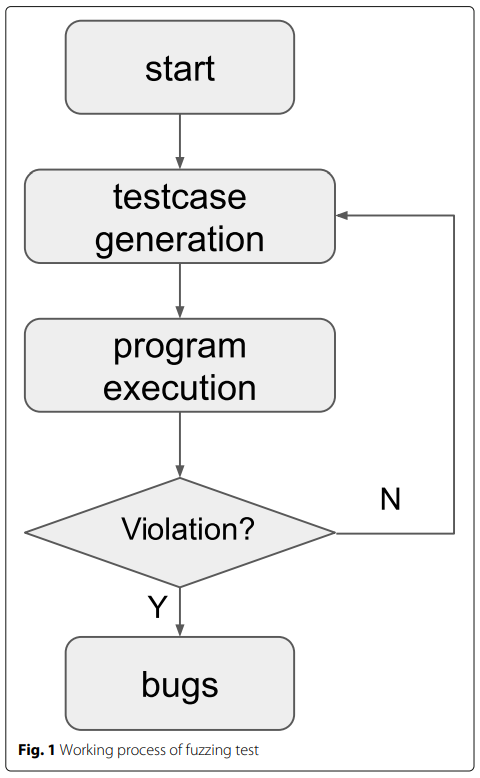
\includegraphics[width=8cm,height=12cm,keepaspectratio]{figuras/fuzzing imagem.png} 
    \legend{Fonte: \href{https://parsif.al}{Fluxograma} (2022, p. TO-DO)}
    \label{fig:internet} 
\end{figure}

O fuzzer generation-based necessita saber como é o input que o programa é capaz de processar. No caso de um fuzzing para arquivos, geralmente é fornecido um arquivo de configuração com o modelo pré-definido de entrada. Os testcases são gerados de acordo com o arquivo de configuração. Fuzzers desse tipo tem facilidade em burlar validações do software testado, permitindo ao pentester entender com mais profundidade a aplicação estudada. Por outro lado, sem uma documentação amigável, analisar o formato do arquivo pode ser uma tarefa árdua.
Em termos de praticidade, fuzzers mutation-based são mais fáceis de utilizar, com aplicabilidade genérica, sendo geralmente o tipo adotado por testes de intrusão no estado da arte. Diferente do generation-based, o mutation-based precisa de alguns inputs iniciais válidos. Os inputs vão sofrendo mutações e novos testcases vão sendo gerados. O wafamole++ requer apenas um input inicial válido - uma query que é fornecida ao final de cada chamada ao comando \verb+wafamole evade+.

Para testes grey box e black box, os fuzzers são mutation-based. Para testes white box, generation-based.

O contexto relevante para o WAF-A-MoLE é produzir, iterativamente, múltiplas injeções SQL a serem testadas a cada "rodada" de mutação. Uma injeção SQL é usada como base inicial, e a mesma sofre mutações por um fuzzer dedicado até ser considerada válida pelo Web Application Firewall testado, embora seja no fundo ainda uma injeção maliciosa. Dessa maneira, o wafamole++ pode ser resumidamente descrito como um fuzzer mutacional, operando em cima de WAFs com entradas de injeções SQL "fuzzeadas".

Referências:

https://www.fuzzingbook.org/html/Fuzzer.html

https://www.fuzzingbook.org/html/MutationFuzzer.html

https://fuzzinginfo.wordpress.com/history/

Fuzzing: a survey, Jun Li, Bodong Zhao and Chao Zhang

https://cybersecurity.springeropen.com/track/pdf/10.1186/s42400-018-0002-y.pdf

\section{Aprendizado de Máquina}
Introduzir conceitos de ML básicos. Melhor ref pra essa intro é \href{link}{https://bibliotecadigital.fgv.br/dspace/handle/10438/30819}. Mencionar POR ALTO (basta nome e descrição bem breve de propósito, métodos e resultados dos algoritmos bases do WAF-A-MoLE (não os novos do wafamole++)):
\begin{alineas}
\item Redes Neurais com Deep Learning - usar artigo Dantas de referência \href{link}{https://bibliotecadigital.fgv.br/dspace/handle/10438/30819}
\item Naive Bayes
\item Random Forest
\item SVM Gaussiana e Linear
\end{alineas}

Mencionar que o resto como é explorado mais a fundo no wafamole++ será descrito nas subseções a seguir com mais detalhes ( Ver parâmetros usados no Cap 4 no wafamole++): 

\subsection{Support Vector Machine}

Usar como ref artigo do Vladimir Vapnik original pra SVM (autor do classificador)

Comentar que modelo novo do wafamole++ é a versão não linear, em contraste com a linear original

\subsection{Stochastic Gradient Descent}

\subsection{Adaboost}

